\chapter{Geometry and Measurement: Part III}

\bigskip
\textit{Distance} is the smallest length between two points. It is an absolute value and is determined by the Pythagorean Theorem. For two points, $P_1$ and $P_2$, the distance is the length $d$, as shown graphically in Figure \ref{fig:distance_graph} below.

\bigskip
A \textit{midpoint} is simply the point between any two given points, and is given by the average of the two points. The coordinate of the midpoint, $M$, of two points, $P_1$ and $P_2$, is shown in Figure \ref{fig:midpoint_graph}.

\vspace{2em}
\begin{figure}[h]
\centering
\begin{minipage}[b]{0.45\textwidth}
\centering
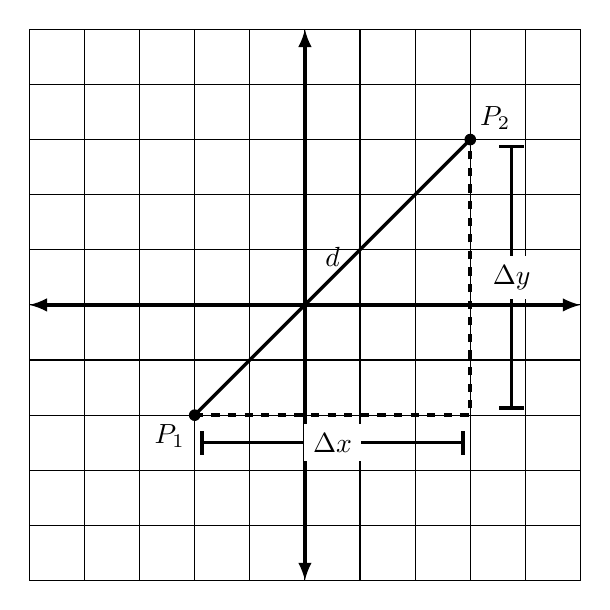
\begin{tikzpicture}[scale=0.7]
\draw (0,0) grid (10,10);
\draw[very thick, latex-latex] (5,0) -- (5,10);
\draw[very thick, latex-latex] (0,5) -- (10,5);
\draw[very thick] (3,3) -- node[midway, above] {$\boldsymbol{d}$} (8,8);
\fill (3,3) circle (3pt) node[below left] {$\boldsymbol{P_1}$};
\fill (8,8) circle (3pt) node[above right] {$\boldsymbol{P_2}$};
\draw[ultra thick, dashed] (3,3) -- (8,3) -- (8,8);
\draw[very thick, |-|] (3.1,2.5) -- node[midway, fill=white] {$\boldsymbol{\Delta x}$}(7.9,2.5);
\draw[very thick, |-|] (8.75,3.1) -- node[midway, fill=white] {$\boldsymbol{\Delta y}$}(8.75,7.9);
\end{tikzpicture}
\caption{Visualization of distance}
\label{fig:distance_graph}
\end{minipage}
\begin{minipage}[b]{0.45\textwidth}
\centering
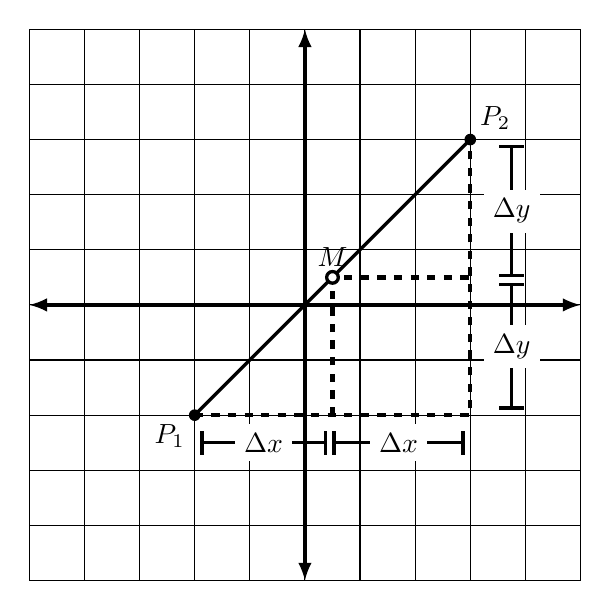
\begin{tikzpicture}[scale=0.7]
\draw (0,0) grid (10,10);
\draw[very thick, latex-latex] (5,0) -- (5,10);
\draw[very thick, latex-latex] (0,5) -- (10,5);
\draw[very thick] (3,3) -- (8,8);
\draw[dashed, ultra thick] (5.5,3) -- (5.5,5.5) -- (8,5.5);
\fill (3,3) circle (3pt) node[below left] {$\boldsymbol{P_1}$};
\fill (8,8) circle (3pt) node[above right] {$\boldsymbol{P_2}$};
\draw[ultra thick, dashed] (3,3) -- (8,3) -- (8,8);
\draw[very thick,fill=white] (5.5,5.5) circle (3pt) node[above] {$\boldsymbol{M}$};
\draw[very thick, |-|] (3.1,2.5) -- node[midway, fill=white] {$\boldsymbol{\Delta x}$}(5.4,2.5);
\draw[very thick, |-|] (5.5,2.5) -- node[midway, fill=white] {$\boldsymbol{\Delta x}$}(7.9,2.5);
\draw[very thick, |-|] (8.75,3.1) -- node[midway, fill=white] {$\boldsymbol{\Delta y}$}(8.75,5.4);
\draw[very thick, |-|] (8.75,5.5) -- node[midway, fill=white] {$\boldsymbol{\Delta y}$}(8.75,7.9);
\end{tikzpicture}
\caption{Visualization of a midpoint}
\label{fig:midpoint_graph}
\end{minipage}
\end{figure}